\usepackage{xcolor}
\usepackage{afterpage}
\usepackage{pifont,mdframed}
\usepackage[bottom]{footmisc}

\makeatletter
\gdef\this@inputfilename{input}
\gdef\this@outputfilename{output}
\makeatother

\newcommand{\funcitem}[2]{\item[$\blacksquare$] \textbf{\large \textsf{Funzione} \texttt{#1}} \vspace{-0.3cm} \begin{center}\begin{tabularx}{\textwidth}{|c|X|} \hline #2 \hline \end{tabularx}\end{center}}

Tra le varie opere di Leonardo, l'affresco raffigurante l'Ultima Cena è considerato uno dei maggiori capolavori. Un amico di Luca sta svolgendo una ricerca approfondita con il compito di fornire una descrizione esaustiva e particolareggiata di queste meraviglie.

Analizzando l'affresco, ha già individuato $N$ ``zone di interesse'' (come quelle racchiuse tra ellissi nella figura sotto), descritte con interi da $1$ a $N$, e $M$ relazioni tra di esse (indicate in figura con delle linee). I motivi per definire una relazione tra due zone sono molti: potrebbero contenere due personaggi che si stanno guardando, oppure due aree dipinte con tecniche similiari oppure completamente opposte, e così via.

\begin{figure}[h]
  \begin{center}
        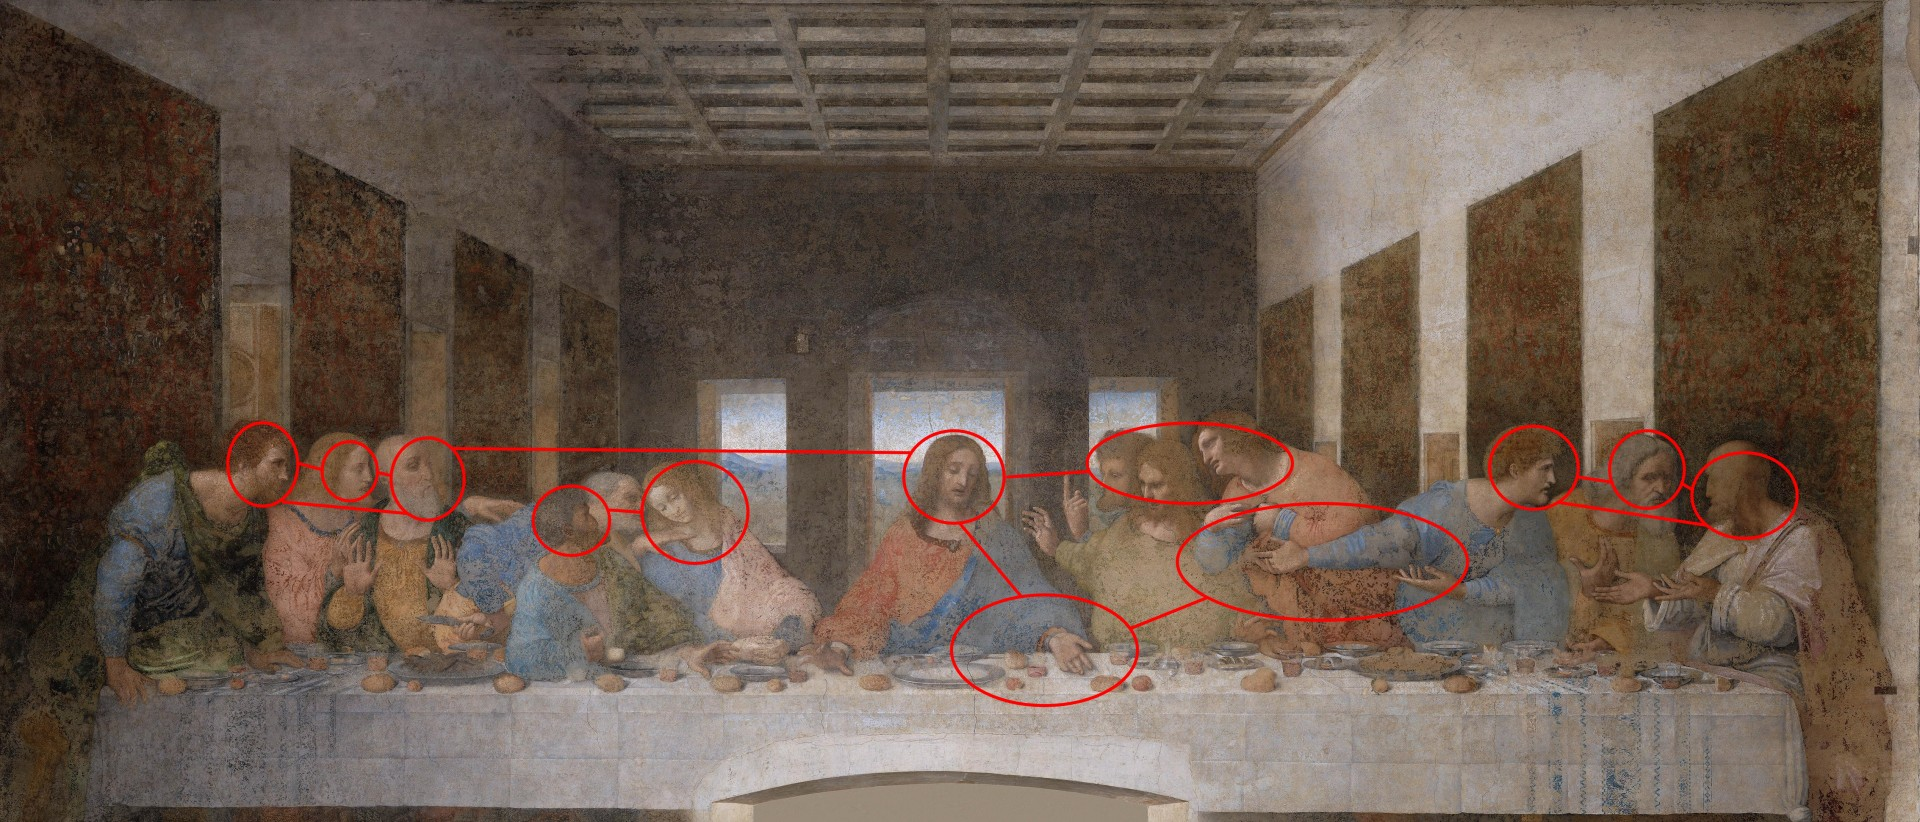
\includegraphics[width=\linewidth]{ultimacena.jpg}
        \caption{Cenacolo vinciano (annotato per evidenziare alcune delle zone di interesse e le loro relazioni).}
  \end{center}
\end{figure}

Il report finale del progetto di ricerca sarà costituito da un elenco delle zone di interesse. Per ognuna verranno descritte, oltre alla zona in sè, anche tutte le relazioni in cui è coinvolta.

Come suo solito, l'amico di Luca è stato particolarmente prolisso e ora il professore a capo del progetto di ricerca non vuole accettare il suo lavoro finché non farà una drastica selezione, includendo al più \textbf{dieci} zone di interesse.

Dopo tutto questo lavoro di accurata descrizione delle relazioni, l'amico è costretto a obbedire al professore ma non vuole sacrificare nemmeno una delle descrizioni già prodotte: aiutalo a selezionare un sottoinsieme $S$ delle $N$ zone in modo che il report finale contenga comunque la descrizione di \emph{tutte} le relazioni!


\Implementation
Dovrai sottoporre un unico file con estensione \texttt{.cpp} o \texttt{.c}.

\begin{warning}
Tra gli allegati a questo task troverai un template (\texttt{ultimacena.cpp} e \texttt{ultimacena.c}) con un esempio di implementazione.
\end{warning}

\pagebreak

Dovrai implementare la seguente funzione:

\begin{itemize}[nolistsep]
    \funcitem{riassumi}{
        C/C++  & \verb|int riassumi(int M, int M, int A[], int B[], int S[]);|\\
    }

    \begin{itemize}[nolistsep]
        \item L'intero $N$ rappresenta il numero delle zone di interesse.
        \item L'intero $M$ rappresenta il numero delle relazioni tra le zone.
        \item Gli array \texttt{A} e \texttt{B}, indicizzati da $0$ a $M-1$, contengono alla posizione $i$ la seguente informazione: esiste una relazione tra le zone \texttt{A[$i$]} e \texttt{B[$i$]}.
        \item La funzione dovrà restituire il numero $S$ di zone da includere nel report finale e riempire l'array \texttt{S} (nelle posizioni da $0$ a $S-1$) con gli identificativi di tali zone.

    \end{itemize}
\end{itemize}

Il grader chiamerà la funzione \texttt{riassumi} in accordo a quanto specificato di seguito.

% % % % % % % % % % % % % % % % % % % % % % % % % % % % % % % % % % % % % % % % % % %
% % % % % % % % % % % % % % % % % % % % % % % % % % % % % % % % % % % % % % % % % % %


\Grader
Allegata a questo problema è presente una versione semplificata del grader usato durante la correzione, che potete usare per testare le vostre soluzioni in locale. Il grader di esempio legge i dati da \texttt{stdin}, chiama la funzione che dovete implementare e scrive su \texttt{stdout}, secondo il seguente formato.

Il file di input è composto da $M+1$ righe, contenenti:
\begin{itemize}[nolistsep,itemsep=2mm]
    \item Riga $1$: gli interi $N$ e $M$, separati da uno spazio.
    \item Righe $2,\ldots, M+1$: i due interi \texttt{A[$i$]} e \texttt{B[$i$]} per $i = 0,\ldots, M-1$.
\end{itemize}

Il file di output è composto da due righe, contenenti:
\begin{itemize}[nolistsep,itemsep=2mm]
    \item Riga $1$: il valore $S$ restituito dalla funzione \texttt{riassumi}.
    \item Riga $2$: i valori contenuti nell'array \texttt{S} (posizioni da $0$ a $S-1$) così come modificato dalla funzione \texttt{riassumi}.
\end{itemize}

% % % % % % % % % % % % % % % % % % % % % % % % % % % % % % % % % % % % % % % % % % %
% % % % % % % % % % % % % % % % % % % % % % % % % % % % % % % % % % % % % % % % % % %

\Constraints

\begin{itemize}[nolistsep, itemsep=2mm]
\item $2 \le N \le 50\,000$.
\item $1 \le M \le 100\,000$.
\item È sempre garantita l'esistenza di una soluzione, ovvero esiste sempre un sottoinsieme costituito da al più dieci zone che rispetta quanto richiesto.
\item Se esistono più soluzioni è possibile stamparne una qualsiasi.
\item L'ordine con cui vengono riportate le zone in una soluzione è irrilevante.
\item Una relazione non viene mai ripetuta in input; inoltre $A_i \neq B_i$ per ogni $i = 0 \ldots M-1$.
\item Ogni zona d'interesse è coinvolta in almeno una relazione.
\end{itemize}

\Scoring
Il tuo programma verrà testato su diversi test case raggruppati in subtask.
Per ottenere il punteggio relativo ad un subtask, è necessario risolvere
correttamente tutti i test relativi ad esso.
\begin{itemize}[nolistsep,itemsep=2mm]
\item \textbf{\makebox[2cm][l]{Subtask 1} [\phantom{0}0 punti]}: Casi d'esempio.
\item \textbf{\makebox[2cm][l]{Subtask 2} [40 punti]}: $N \le 15$.
\item \textbf{\makebox[2cm][l]{Subtask 3} [40 punti]}: $N \le 1000$.
\item \textbf{\makebox[2cm][l]{Subtask 4} [20 punti]}: Nessuna limitazione specifica.
\end{itemize}

\Examples
\begin{example}
\exmpfile{ultimacena.input0.txt}{ultimacena.output0.txt}%
\exmpfile{ultimacena.input1.txt}{ultimacena.output1.txt}%
\end{example}

\Explanation

Nel \textbf{primo caso di esempio} le zone di interesse sono così poche da poter essere incluse tutte nel report senza problemi. Naturalmente sarebbe stato ammissibile produrre soluzioni diverse (ad esempio includendo le sole zone 3 e 4).


Nel \textbf{secondo caso di esempio} ci sono $11 > 10$ zone di interesse, quindi dobbiamo escluderne (almeno) una. Possiamo escludere la zona 1, le cui uniche relazioni sono con le zone 3 e 4 già incluse nel report finale.
